\chapter{Terceiro Projeto: Sistema para Venda de Produtos}\label{cap:terceiroProjeto}
\epigraph{``\textit{A imaginação é mais importante que o conhecimento}''.}{Albert Einstein}

\lettrine[lines=4, lhang=0.1, lraise=0, loversize=0.2, findent=0.1em]{\textcolor{corTema}{N}}{ESTE} Capítulo iremos construir mais um projeto completo, concluindo o aprendizado dos conhecimentos básicos para que você possa construir praticamente qualquer tipo de sistema que lide com bancos de dados relacionais, ou seja, aprenderemos a lidar com a implementação de cadastros que têm relacionamentos ``muitos-para-muitos''.


\section{Introdução}

Finalmente estamos aptos a construir uma aplicação Web em Java com a maioria das funcionalidades necessárias à maioria das aplicações Web que você desenvolverá na sua vida profissional. Iremos incrementar a aplicação criada no Capítulo~\ref{cap:primeiroProjeto} desenvolvendo mais alguns cadastros e amarrando todos eles em um cadastro de vendas de produtos. Vamos lá!

Além de clientes, cidades e estados, criaremos mais três cadastros com inserção, alteração e remoção de registros: unidades de medida, produtos e fornecedores. Com esses seis cadastros desenvolveremos a interface gráfica das vendas, onde poderemos gerar novas vendas e que, após serem feitas, poderão ser canceladas.

Na Figura~\ref{fig:cap08ModeloFisico} pode ser visto o modelo físico da base de dados \texttt{venda\_produtos}. Note que o nome da base é diferente do projeto anterior. Para esse projeto o \textit{script} SQL para a criação da base de dados não será fornecido pois, além da estrutura, teremos algumas inserções já prontas para podermos testar. Para gerar a base, com o MariaDB/MySQL em execução, abra o modelo da base no MySQL Workbench, disponibilizado nos arquivos do Capítulo. Com o modelo aberto, clique no menu \destaque{\textit{Database}} escolha a opção \destaque{\textit{Forward Engineer...}} e siga o assistente. A base de dados, as tabelas e os relacionamentos serão criados, além de várias inserções para as tabelas estado, cidade, cliente, fornecedor, unidade\_medida e produto que serão realizadas.

\FloatBarrier
\begin{figure}[!htbp]
    \centering
    \caption{Diagrama do modelo físico da base de dados}
    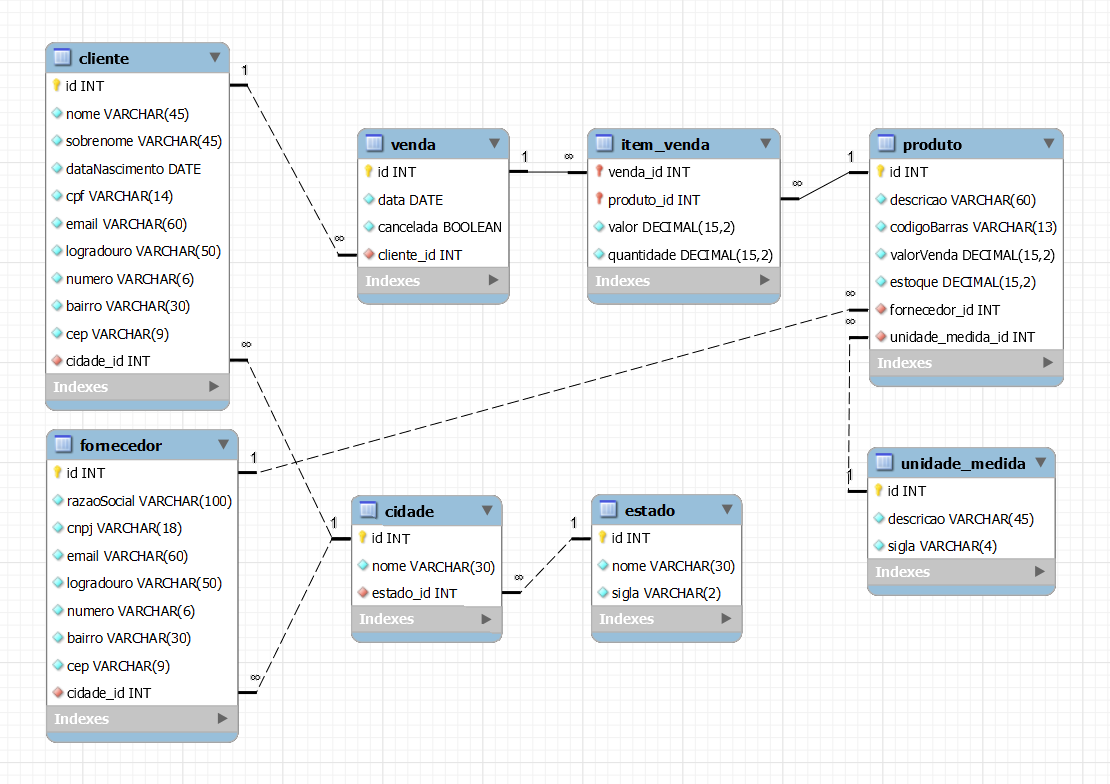
\includegraphics[scale=0.5]{imagens/cap08ModeloFisico}
    \\\textbf{Fonte:} Elaborada pelo autor
    \label{fig:cap08ModeloFisico}
\end{figure}
\FloatBarrier

O diagrama de classes das entidades do projeto pode ser visto Figura~\ref{fig:cap08DiagramaClasses}. Veja que a classe \texttt{ItemVenda} é a classe que fará o papel de viabilizar o relacionamento muitos-para-muitos entre produtos e vendas. Note que na UML existe a notação de classe associativa que poderia ter sido usada para representar esse relacionamento.

\FloatBarrier
\begin{figure}[!htbp]
    \centering
    \caption{Diagrama de classes das entidades}
    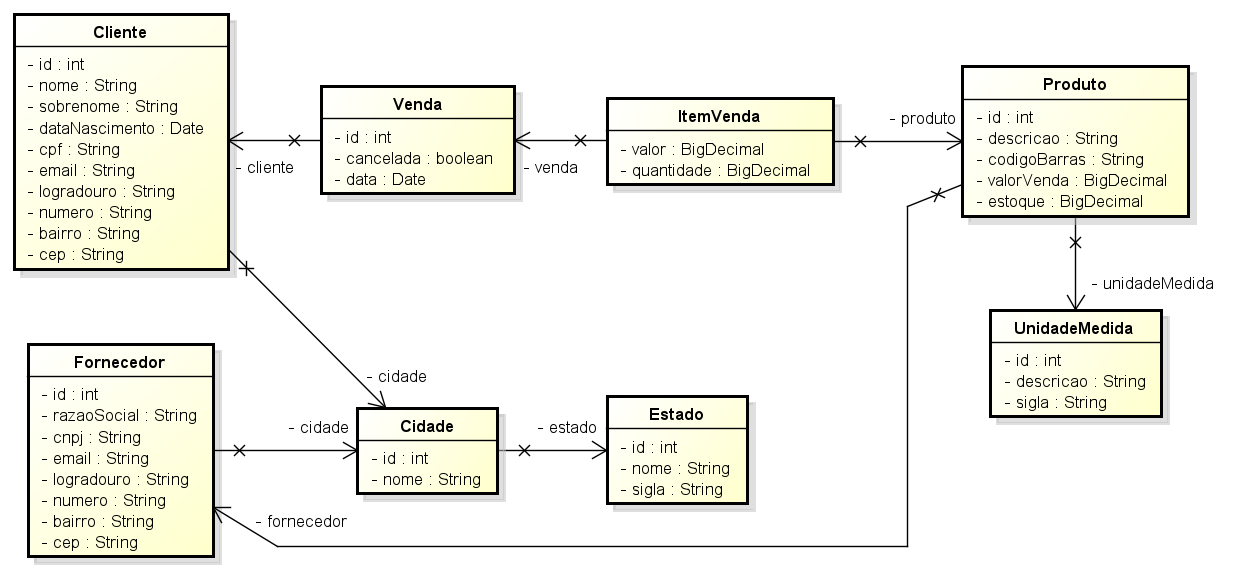
\includegraphics[scale=0.45]{imagens/cap08DiagramaClasses}
    \\\textbf{Fonte:} Elaborada pelo autor
    \label{fig:cap08DiagramaClasses}
\end{figure}
\FloatBarrier

Para que esse Capítulo não fique gigantesco, focaremos apenas nas novidades ou modificações que foram feitas em relação ao projeto anterior. Você poderá pegar o projeto pronto nos arquivos do Capítulo. A entidade \texttt{Produto} será usada como base para entendermos o que foi alterado e depois toda a parte da venda propriamente dita será detalhada com mais afinco.


\section{Construindo o Sistema}

Esta seção será dividida em várias subseções para que possamos organizar o que foi modificado em relação ao sistema anterior além, é claro, das funcionalidades novas. Os seis cadastros base são similares, então apenas um, como já explicado, será detalhado e o restante é por sua conta dar uma olhada, bastando consultar o código pronto no projeto disponibilizado.


\subsection{Entidades e Validações}

Começaremos discutindo nossas entidades. Todos os membros de todas elas agora serão de tipos de referência, ou seja, qualquer tipo que não seja primitivo. Os membros de tipo \inlineJavaCode{int}, que usamos anteriormente para definir os identificadores, passarão a ser do tipo \texttt{Long}. Todos os tipos numéricos decimais serão do tipo \texttt{BigDecimal}, principalmente quando precisarmos representar valores monetários, fugindo assim da imprecisão dos tipos de ponto flutuante, pois dinheiro é algo muito importante e precisamos tomar muito, muito, MUITO cuidado com esse tipo de dado em um sistema de verdade. Além disso, cada atributo será anotado com pelo menos uma anotação de validação, pois todos os nossos objetos das entidades serão validados, obrigatoriamente antes de serem submetidos aos seus respectivos DAOs, filtrando possíveis tentativas de adulteração dos dados submetidos através dos formulários. Na entidade \texttt{Produto}, apresentada na Listagem~\thechapter.\ref{listagem:projetos/capitulo08/VendaProdutos/src/java/vendaprodutos/entidades/Produto.java}, podemos ver isso.

\javaCode{Entidade ``Produto''\newline%
Arquivo: \texttt{vendaprodutos/entidades/Produto.java}}{projetos/capitulo08/VendaProdutos/src/java/vendaprodutos/entidades/Produto.java}

Sempre precedendo a definição de um atributo da classe utilizaremos essas anotações. Na linha 17 o atributo identificador da entidade \texttt{Produto} é declarado e, logo antes, na linha 16, é usada a anotação \inlineJavaCode{@NotNull} que indica que um objeto do tipo \texttt{Produto}, ao ser validado, não poderá ter esse atributo configurado com \inlineJavaCode{null}. Veremos o mecanismo de validação já, já. O atributo \texttt{descricao} é anotado com \inlineJavaCode{@NotNull}, que já aprendemos, e \inlineJavaCode{@Size} que, dependendo do tipo, verificará o tamanho do valor do mesmo. Para \texttt{Strings}, que é o nosso caso, é a quantidade de caracteres. Na linha 20 temos então que a descrição dos produtos pode ter no mínimo um caracetere e no máximo 60. Note que todas as nossas validações serão consistentes com as restrições existentes no modelo físico do banco de dados. O código de barras de um produto terá obrigatoriamente que bater com um padrão de 13 dígitos, usando para isso a anotação \inlineJavaCode{@Pattern} com o atributo \texttt{regexp} (\textit{regular expression}). Essa expressão regular diz que o padrão deve casar com a String inteira, sendo que isso é indicado pelos meta-símbolos \^{} e \$ que significam, respectivamente, início e fim da \texttt{String}. O méta-símbolo \textbackslash{}d significa um dígito ($0$ a $9$) e há a necessidade de se usar duas contrabarras, pois como em Java a contrabarra indica um caracetere de escape, precisamos usar duas para escapá-la. O atributo \texttt{message} de \inlineJavaCode{@Pattern} é usado para criarmos uma mensagem personalizada para quando o produto for validado e esse atributo estiver fora do que é esperado.

A anotação \inlineJavaCode{@PositiveOrZero} indica que o atributo do tipo \texttt{BigDecimal} deve ser zero ou qualquer valor positivo. As outras anotações que usaremos nas outras entidades são \inlineJavaCode{@Positive} para valores positivos obrigatoriamente (zero não é positivo nem negativo!) e \inlineJavaCode{@Email} para verificar se o valor representa um formato válido de e-mail. A implementação de referência da \textit{Jakarta Bean Validation} faz parte do Jakarta EE 8, que estamos usando, e é fornecida pelo Hibernate Validator.

\begin{saibaMais}
    O site oficial da especificação e da implementação da API \textit{Bean Validation} pode ser acessada pelo link \url{https://beanvalidation.org/}
\end{saibaMais}

A validação dos objetos será feita sempre nos Servlets e é implementada pelo método \inlineJavaCode{validar}, que tem sua implementação iniciada na linha 187 da classe \texttt{Utils}, mostrada na Listagem~\thechapter.\ref{listagem:projetos/capitulo08/VendaProdutos/src/java/vendaprodutos/utils/Utils.java}.

\javaCode{Classe ``Utils'' com métodos estáticos utilitários\newline%
Arquivo: \texttt{vendaprodutos/utils/Utils.java}}{projetos/capitulo08/VendaProdutos/src/java/vendaprodutos/utils/Utils.java}

Na nossa implementação da validação de objetos forneceremos a opção do usuário do método ignorar a validação de atributos de uma classe, caso seja necessário. Por exemplo, um \texttt{Produto} novo não terá identificador até que seja persistido, mas precisaremos validá-lo antes de ser enviado ao seu DAO. O método validar faz uso do método estático privado \inlineJavaCode{validarObj} que é quem invoca de fato a infraestrutura de validação. Veja o código, está todo comentado. O método \inlineJavaCode{validar} lançará uma exceção do tipo \texttt{SQLException} caso o objeto seja inválido e essa exceção terá encapsulada como mensagem a descrição de todas as inconsistências identificadas no objeto. Essa mensagem será configurada com uma série de \textit{tags} \inlineHTMLCode{<li>} e será usada na página de erros da aplicação. Veremos essa questão da página de erros mais adiante no Capítulo.

Vamos ver agora o que mudou na nossa camada de persistência.


\subsection{DAO}

Temos duas novidades na nossa camada de persistência. A primeira é a implementação da interface \texttt{AutoCloseable} que permitirá que usemos objetos dos nossos DAOs na construção \textit{try-with-resources} que, por sua vez, fará o fechamento automático da conexão dos DAOs ao terminarem de serem utilizados. Para isso precisaremos implementar o método \inlineJavaCode{close} que substituirá o nosso antigo \inlineJavaCode{fecharConexao}. A implementação do DAO genérico é mostrada na Listagem~\thechapter.\ref{listagem:projetos/capitulo08/VendaProdutos/src/java/vendaprodutos/dao/DAO.java}, sendo que o método \inlineJavaCode{close} pode ser visto entre as linhas 57 e 59.

\javaCode{DAO genérico\newline%
Arquivo: \texttt{vendaprodutos/dao/DAO.java}}{projetos/capitulo08/VendaProdutos/src/java/vendaprodutos/dao/DAO.java}

A outra mudança que temos em nossos DAOs é que agora, toda entidade que tiver um objeto submetido ao método \inlineJavaCode{salvar(...)}, será modificada para conter o identificador que foi gerado pelo SGBD. Na Listagem~\thechapter.\ref{listagem:projetos/capitulo08/VendaProdutos/src/java/vendaprodutos/dao/ProdutoDAO.java} é apresentado o DAO para produtos.

\javaCode{Código da classe ``ProdutoDAO''\newline%
Arquivo: \texttt{vendaprodutos/dao/ProdutoDAO.java}}{projetos/capitulo08/VendaProdutos/src/java/vendaprodutos/dao/ProdutoDAO.java}

Veja que a criação do \texttt{PreparedStatement} do método \inlineJavaCode{salvar(...)} agora usa outra versão do método \inlineJavaCode{prepareStatement(...)} de \texttt{Connection}. Nessa versão, além da \texttt{String} contendo o código SQL que será executado, é passado um array de \texttt{Strings} com o nome da ou das colunas que representam as chaves primárias daquela tabela. Essa ``artimanha'' funciona para colunas que são auto-incrementáveis, que é o caso dos nossos identificadores. Precisaremos dessa característica no cadastro das vendas. Veremos isso mais para frente. Quando fazemos uso desse recurso, após a persistência do objeto, que gerará uma nova linha/registro/tupla na tabela, precisaremos usar o mesmo \texttt{PreparedStatement} para obter a ou as chaves. Isso será feito no método \inlineJavaCode{getChavePrimariaAposInsercao(...)} da classe \texttt{Utils} (linha 133 da Listagem~\thechapter.\ref{listagem:projetos/capitulo08/VendaProdutos/src/java/vendaprodutos/utils/Utils.java}). Como consistentemente estamos usando uma coluna chamada \texttt{id} como chave primária auto-incrementável, usaremos esse método para todas as nossas entidades, com exceção da \texttt{ItemVenda} que funcionará de outra forma.

Muito bem, temos nossas entidades prontas para serem validadas e a camada de persistência atualizada. Vamos ver agora o que mudou nos nossos Servlets.


\subsection{Servlets}

Nossos Servlets continuarão a funcionar e a ter a mesma estrutura que vimos anteriormente, mas agora com algumas melhorias. Na Listagem~\thechapter.\ref{listagem:projetos/capitulo08/VendaProdutos/src/java/vendaprodutos/controladores/ProdutosServlet.java} pode ser visto o código completo do Servlet de produtos.

\javaCode{Código-fonte do Servlet ``ProdutosServlet''\newline%
Arquivo: \texttt{vendaprodutos/controladores/ProdutosServlet.java}}{projetos/capitulo08/VendaProdutos/src/java/vendaprodutos/controladores/ProdutosServlet.java}

As ações esperadas dos formulários serão as mesmas. Entre as linhas 37 e 39 instanciamos três DAOs, um para produtos, um para fornecedores e um para unidades de medida. Precisaremos dos dois últimos para trazer do banco de dados os objetos necessários para compor o produto.

A partir da linha 43 iniciam-se as instruções para obtenção dos dados do formulário de criação/inserção de um novo produto. Veja que entre as linhas 45 e 52 usamos os métodos \inlineJavaCode{getBigDecimal(...)} e \inlineJavaCode{getLong(...)} para a obtenção dos dados numéricos que virão do formulário. Estamos prevendo o caso de haver alguma inserção incorreta, passando a validação do lado do cliente e, nesses métodos, que estão definidos respectivamente nas linhas 42 e 61 da Listagem~\thechapter.\ref{listagem:projetos/capitulo08/VendaProdutos/src/java/vendaprodutos/utils/Utils.java}, é feita a obtenção dos valores e, caso haja algum problema, eles retornarão \inlineJavaCode{null} ao invés de lançar exceção. Nas linhas 54 e 55 usamos os DAOs dos fornecedores e unidades de medida para a obtenção dos objetos que contém os \texttt{ids} que vieram do formulário. Entre as linhas 57 e 63 configuramos todos os atributos do novo produto que será inserido e, na linha 65, antes de ``salvarmos'' o objeto no banco de dados, realizamos a validação. Note que estamos ignorando o atributo \texttt{id}, pois um novo produto ainda não o tem. O método de validação lançará uma \texttt{SQLException} caso haja algum erro na validação e, caso tudo esteja correto, o produto será salvo na linha 66 e na linha 67 preparamos o despacho para voltar à página de listagem. Outra coisa, após a execução do método \inlineJavaCode{salvar(...)} do DAO de produtos, o produto terá seu identificador configurado. Nesse caso não fará muita diferença, mas precisaremos desse comportamento da obtenção do \texttt{id} gerado pelo auto-incremento quando formos lidar com as vendas.

O restante dos tratamentos das ações dos formulários continuam praticamente as mesmas. Como nossos DAOs foram instanciados usando um \textit{try-with-resources}, não precisamos fechar as conexões dos DAOs de forma explícita, simplificando um pouco nosso código. Caso haja qualquer problema de validação ou mesmo em nível do SGBD, a \texttt{SQLException} lançada será capturada no \inlineJavaCode{catch} da linha 125. Ali usamos mais um método da classe \texttt{Utils}, definido na linha 218 da Listagem~\thechapter.\ref{listagem:projetos/capitulo08/VendaProdutos/src/java/vendaprodutos/utils/Utils.java}, em que preparamos o redirecionamento para a página de erros do nosso sistema. Note que na linha 223 da classe \texttt{Utils} configuramos um atributo do \textit{request} com o nome de \texttt{mensagemErro}, em que a mensagem da exceção será usada e na linha 224 configuramos o segundo parâmetro, chamado \texttt{voltarPara}, em que obtemos de qual recurso que veio a requisição para o Servlet, usando para isso o cabeçalho \texttt{Referer} da requisição, permitindo que criemos o \textit{link} apropriado para que possamos voltar à página de onde o erro foi gerado.

Por falar em erros, na Listagem~\thechapter.\ref{listagem:projetos/capitulo08/VendaProdutos/web/erro.jsp} pode ser visto o arquivo JSP que tratará os erros de validação e de persistência do sistema.

\htmlCode{Página para exibição de erros\newline%
Arquivo: \texttt{/erro.jsp}}{projetos/capitulo08/VendaProdutos/web/erro.jsp}

Com o conhecimento que você já adquiriu com o que estamos trabalhando você será capaz de entender o que essa página faz.


\subsection{Cadastro de Vendas}

Agora vamos detalhar todo o cadastro de vendas do sistema onde, de certa forma, todos os cadastros básicos convergirão. Começaremos com o lado do servidor, o chamado \textit{back-end}.

\subsubsection{\textit{Back-End}}

Na Listagem~\thechapter.\ref{listagem:projetos/capitulo08/VendaProdutos/src/java/vendaprodutos/entidades/Venda.java} pode ser vista a entidade \texttt{Venda}. Uma venda só poderá ser cadastrada e, caso necessário, ser cancelada. Estamos tentando simular um sistema real com anotações fiscais e esse tipo de coisa precisa acontecer, ou seja, uma venda nunca deve ser excluída! Para o tratamento do cancelamento temos o atributo \texttt{cancelada}.

\javaCode{Entidade ``Venda''\newline%
Arquivo: \texttt{vendaprodutos/entidades/Venda.java}}{projetos/capitulo08/VendaProdutos/src/java/vendaprodutos/entidades/Venda.java}

Na Listagem~\thechapter.\ref{listagem:projetos/capitulo08/VendaProdutos/src/java/vendaprodutos/entidades/ItemVenda.java} a entidade \texttt{ItemVenda} é apresentada. 

\javaCode{Entidade ``ItemVenda''\newline%
Arquivo: \texttt{vendaprodutos/entidades/ItemVenda.java}}{projetos/capitulo08/VendaProdutos/src/java/vendaprodutos/entidades/ItemVenda.java}

Cada venda pode conter um ou mais produtos que, por sua vez, podem ter sido vendidos em uma ou mais vendas, sendo assim, precisamos ter uma entidade que associa as outras duas. O valor do item da venda é o valor do produto naquele momento em que foi vendido, visto que o valor de venda de um produto pode variar com o tempo, mas o valor usado no momento da venda deve ser mantido! Além disso, todo item da venda tem uma quantidade associada, pois podemos ter comprado, por exemplo, duas caixas de ovos ou um quilo e meio de peito de frango.

O código do DAO que trata as vendas é apresentado na Listagem~\thechapter.\ref{listagem:projetos/capitulo08/VendaProdutos/src/java/vendaprodutos/dao/VendaDAO.java}. O método \inlineJavaCode{atualizar(...)} será usado para cancelar uma venda. Além disso, não há razão para excluirmos vendas realizadas, sendo assim, o corpo do método está vazio.

\javaCode{Código da classe ``VendaDAO''\newline%
Arquivo: \texttt{vendaprodutos/dao/VendaDAO.java}}{projetos/capitulo08/VendaProdutos/src/java/vendaprodutos/dao/VendaDAO.java}

Já o \texttt{ItemVendaDAO} é exibido na Listagem~\thechapter.\ref{listagem:projetos/capitulo08/VendaProdutos/src/java/vendaprodutos/dao/ItemVendaDAO.java}.

\javaCode{Código da classe ``ItemVendaDAO''\newline%
Arquivo: \texttt{vendaprodutos/dao/ItemVendaDAO.java}}{projetos/capitulo08/VendaProdutos/src/java/vendaprodutos/dao/ItemVendaDAO.java}

Nesse DAO temos a implementação do método \inlineJavaCode{salvar(...)}, mas a atualização, a exclusão, a obtenção de todos os itens de venda e a obtenção por \texttt{id} não são implementadas, visto que nunca mexeremos numa venda após ser feita, mas como poderemos cancelar uma venda, implementamos um método adicional no \texttt{ItemVendaDAO} chamado de \inlineJavaCode{obterPorIdVenda}, definido a partir da linha 80. Esse método retornará todos os itens de uma determinada venda para que, ao haver a necessidade de cancelá-la, possamos atualizar o estoque dos produtos, pois se uma venda foi cancelada, os produtos deverão ser devolvidos à loja e voltarão a compor o estoque.

Vamos agora fechar a implementação do nosso \textit{back-end} detalhando o Servlet das vendas. Na Listagem~\thechapter.\ref{listagem:projetos/capitulo08/VendaProdutos/src/java/vendaprodutos/controladores/VendasServlet.java} pode ser visto o código completo do mesmo.

\javaCode{Código-fonte do Servlet ``VendasServlet''\newline%
Arquivo: \texttt{vendaprodutos/controladores/VendasServlet.java}}{projetos/capitulo08/VendaProdutos/src/java/vendaprodutos/controladores/VendasServlet.java}

Esse Servlet tratará dois tipos de ação. Uma de inserção, entre as linhas 55 e 106 e uma de cancelamento, entre as linhas 110 e 130. A inserção de uma venda envolve a associação do cliente que está comprando do estabelecimento, a data da mesma e todos os itens que a compõe. Veja que a variável \texttt{itensVenda} é uma \texttt{String} que conterá dados codificados em JSON que virão do cliente. Precisaremos processar esse JSON do lado do servidor parar criar um objeto genérico que conterá o ou os identificadores do produtos e a ou as respectivas quantidades vendidas. O processo de construção desse JSON será visto quando formos tratar sobre o lado do cliente. Veremos isso logo.

Veja que o processamento do JSON dos itens da venda é feito inicialmente criando um objeto do tipo \texttt{JsonReader} nas linhas 60 e 61. Posteriormente, na linha 63 o processo de \textit{parsing} do JSON é feito, atribuindo o resultado à variável \inlineJavaCode{jsaItensVenda} do tipo \texttt{JsonArray}. Após salvarmos a venda na linha 73, iteraremos sobre \inlineJavaCode{jsaItensVenda} para extrairmos cada objeto genérico com os dados que precisamos para ``amarrar'' os produtos vendidos na venda realizada. Essa iteração ocorre entre as linhas 76 e 103, onde inicialmente obtemos o objeto genérico atual (linha 79), extraímos os dados necessários entre as linhas 82 e 85 e na linha 88 consultamos o produto e atualizamos o seu estoque (só no objeto por enquanto), visto que como estamos vendendo, precisamos subtrair a quantidade do estoque. Entre as linhas 92 e 96 criamos o item da venda, na linha 100 atualizamos o produto por causa do estoque (agora no banco de dados) e na linha 101 salvamos o item da venda. Não precisamos validar os itens de venda nem os produtos, visto que todo esse processamento será feito internamente.

O processo de cancelamento, tratado entre as linhas 110 e 130, atualizará a venda, marcando-a como cancelada e atualizará os estoques dos produtos associados. Note que não criaremos um \texttt{RequestDispatcher}, pois a ação de cancelamento será executada via AJAX. Não trataremos situações em que possam haver problemas no SGBD, pois após o cancelamento de uma venda retornaremos um JSON sinalizando que a requisição foi bem sucedida, mas em um sistema mais robusto teríamos que pensar nisso também. Uma outra coisa a se pensar, mas que não foi endereçada na nossa implementação, seria o caso de haver algum erro durante a inserção dos itens de venda ou na atualização dos produtos no cancelamento. Isso seria resolvido configurando o driver do SGBD para que as transações fossem gerenciadas manualmente e iniciadas antes das operações dos DAOs e finalizadas explicitamente com um \textit{commit} caso tudo ocorresse como esperado ou canceladas (\textit{rollback}) na detecção de algum problema.

Algo importante que não lidamos na nossa implementação é o caso de algum problema acontecer durante o processo de atualização vários tantos registros na base de dados. Imagine se o primeiro item de venda foi processado corretamente, mas no segundo, por algum motivo, aconteceu algum erro como o servidor perdeu a comunicação com o SGBD. Se isso acontecer, teremos dados corrompidos, pois o que deveria ter sido feito completamente foi feito parcialmente, concorda? Por exemplo, no caso de inserção/cadastro, o ideal seria iniciarmos uma transação antes de salvar a venda e dar um ``\textit{commit}'' nessa transação antes encaminharmos a requisição para a página de listagem, ou dar um ``\textit{rollback}'' em caso de algum problema acontecer, desfazendo o que foi feito desde o início da transação, evitando problemas na estrutura da base de dados que foi modificada. Novamente, para simplificarmos um pouco mais a implementação isso não foi endereçado. Trataremos esse tipo de situação no Capítulo de persistência, tudo bem?

Vamos agora tratar o lado do cliente.


\subsubsection{\textit{Front-End}}

Começaremos conferindo como a listagem das vendas foi implementada. Basicamente ela consiste na mesma estrutura dos outros cadastros, ou seja, uma \inlineHTMLCode{<table>} em que cada linha há um registro da tabela do banco de dados em questão. Estamos fazendo a construção dessa tabela a partir das classes de serviços, você se lembra? A novidade aqui é que uma venda não pode ser excluída ou atualizada, com a exceção de que ela pode ser cancelada. O cancelamento será feito através de uma chamada em AJAX. Para implementarmos isso, veja o \inlineHTMLCode{<c:choose>} construído entre as linhas 60 e 69 da Listagem~\thechapter.\ref{listagem:projetos/capitulo08/VendaProdutos/web/formularios/vendas/listagem.jsp}.

\htmlCode{Código da listagem de Vendas\newline%
Arquivo: \texttt{/formularios/vendas/listagem.jsp}}{projetos/capitulo08/VendaProdutos/web/formularios/vendas/listagem.jsp}

Caso uma venda esteja cancelada, a palavra ``Cancelada'' aparecerá na coluna de cancelamento. Caso contrário, entre as linhas 65 e 67, será gerado um \textit{link} apontando para ``\texttt{\#}'' no atributo \texttt{href}, sendo que o sinal ``\texttt{\#}'' sozinho indica que é uma âncora para lugar nenhum, ou seja, quando o \textit{link} for clicado, ele não fará nada. Outras \textit{tags} poderiam ter sido usadas aqui, mas para manter a consistência na GUI em relação aos outros cadastros, optei por usar \textit{hyperlinks} mesmo. Nosso \textit{link} terá mais dois atributos definidos. Um você já conhece, que é o \texttt{onclick}, apontando para a função \inlineJavaScriptCode{cancelarVenda(...)}. O outro é o atributo \texttt{data}. Esse atributo é interessante pois podemos armazenar dados nas \textit{tags}! Para usá-lo, começamos com a palavra \texttt{data}, inserimos um traço e depois um identificador qualquer, sem espaços ou letras maiúsculas. Caso queira um identificador com nome composto, ou seja, com mais de uma palavra, separe-as por traços. No nosso caso, o identificador é \texttt{id}. A ideia é que esse \textit{link} tenha um dado associado que é o identificador da venda. A função \inlineJavaScriptCode{cancelarVenda(...)} usará esse dado para saber qual venda deve ser cancelada. Note que também poderíamos ter passado o identificador da venda como argumento para a função, mas eu quis usar o atributo \texttt{data} para vocês saberem que ele existe.

\begin{saibaMais}
    Mais sobre os atributos \texttt{data}: \url{https://developer.mozilla.org/en-US/docs/Learn/HTML/Howto/Use_data_attributes}
\end{saibaMais}

Vamos dar uma olhada no arquivo de \textit{script} em que a função \inlineJavaScriptCode{cancelarVenda(...)} está implementada. Esse arquivo pode ser visto na Listagem~\thechapter.\ref{listagem:projetos/capitulo08/VendaProdutos/web/js/formularios/vendas/listagem.js}.

\javaScriptCode{\textit{Script} para cancelamento de Vendas\newline%
Arquivo: \texttt{/js/formularios/vendas/listagem.js}}{projetos/capitulo08/VendaProdutos/web/js/formularios/vendas/listagem.js}

Dentro da função temos a implementação da requisição AJAX feita tanto usando JavaScript puro, empregando a Fetch API entre as linhas 7 e 26, quanto usando jQuery, implementação essa que está comentada e é encontrada entre as linhas 29 e 46. Na linha 5 obtemos o identificador da venda através do atributo \texttt{dataset}, que é quem referencia os atributos \texttt{data} definidos no código HTML. Veja que acessamos o atributo \texttt{target} do evento, que representa quem disparou o evento, no caso o \textit{link} que foi clicado, acessamos o atributo \texttt{dataset} do \textit{link} e, por sua vez, o atributo \texttt{id} do \texttt{dataset}, que é quem está armazenando o dado que queremos, ou seja, o identificador da venda armazenado no banco de dados. Novamente, como já foi dito, poderíamos alternativamente ter passado o identificador da venda em um parâmetro dessa função.

Nossa requisição AJAX aponta para o Servlet de vendas, mapeado na URL\newline%
\texttt{/processaVendas}. Note que passamos o contexto da aplicação para a função, evitando problemas de referências quebradas. Veja que quando a requisição for feita, a ação ``cancelar'' será processada no Servlet, atualizando a coluna do registro que indica que a venda está cancelada, além de retornar ao estoque do ou dos produtos vendidos as suas respectivas quantidades. Note que em caso de sucesso, o JSON trazido do servidor será processado na linha 15 e então o objeto criado, chamado de data, será utilziado para verificar o status, que no caso só poderá ser ``ok'', e o conteúdo da célula da tabela onde a \textit{tag} \inlineHTMLCode{<a>} existia (\texttt{parentElement}) será atualizado para ``Cancelada'', não permitindo mais ser clicado, pois a partir desse momento não haverá mais um \textit{link} naquela posição.

Agora trataremos o nosso formulário de cadastro de uma nova venda. Esse formulário é um pouco mais elaborado que os anteriores, sendo que podemos ver seu código completo na Listagem~\thechapter.\ref{listagem:projetos/capitulo08/VendaProdutos/web/formularios/vendas/novo.jsp}.

\htmlCode{Formulário de cadastro de novas Vendas\newline%
Arquivo: \texttt{/formularios/vendas/novo.jsp}}{projetos/capitulo08/VendaProdutos/web/formularios/vendas/novo.jsp}

Graficamente, o código acima gerará algo como apresentado na Figura~\ref{fig:cap08FormularioNovaVenda}.

\FloatBarrier
\begin{figure}[!htbp]
    \centering
    \caption{Formulário para Novas Vendas}
    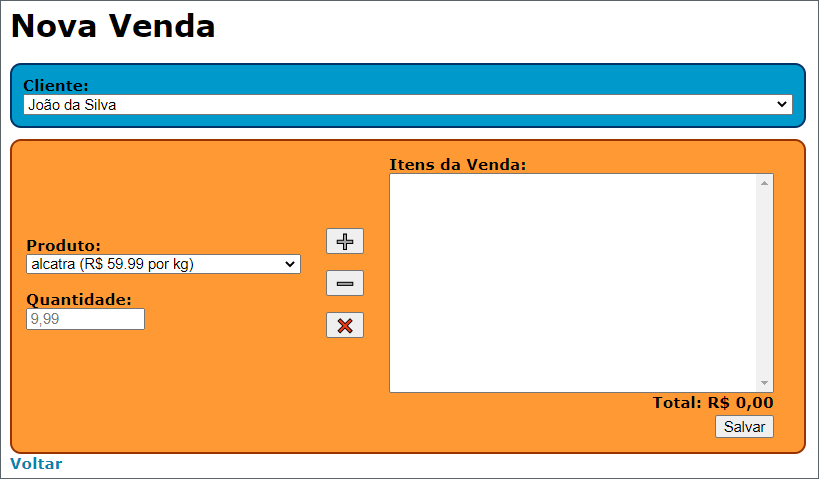
\includegraphics[scale=0.7]{imagens/cap08FormularioNovaVenda}
    \\\textbf{Fonte:} Elaborada pelo autor
    \label{fig:cap08FormularioNovaVenda}
\end{figure}
\FloatBarrier

Você já conhece praticamente todo o código utilizado na Listagem~\thechapter.\ref{listagem:projetos/capitulo08/VendaProdutos/web/formularios/vendas/novo.jsp}, sendo assim focaremos na implementação da funcionalidade apresentado na Listagem~\thechapter.\ref{listagem:projetos/capitulo08/VendaProdutos/web/js/formularios/vendas/novo.js}.

\javaScriptCode{\textit{Script} para tratamento de novas Vendas\newline%
Arquivo: \texttt{/js/formularios/vendas/novo.js}}{projetos/capitulo08/VendaProdutos/web/js/formularios/vendas/novo.js}

Neste formulário optei por fazer o registro de todos os eventos programaticamente. Na linha 6 usamos um dialeto padrão da jQuery em que registramos uma função, passada como argumento para a função \inlineJavaScriptCode{$(...)}, como ouvinte do ``evento'' \texttt{onready}. Esse evento na verdade é uma construção da biblioteca jQuery que define que quando o documento está pronto, ou seja, todo o HTML já passou pelo processo de \textit{parsing} pelo navegador, a função será executada, o que é diferente do evento \texttt{onload} da \textit{tag} \inlineHTMLCode{<body>} que é disparado quando todo o HTML e todos os recursos como imagens, arquivos externos etc. forem carregados. Note que essa função contém todas as outras que vamos usar.

Na linha 9 criamos um array que armazenará todos os itens da venda que iremos montar durante o uso do formulário. Entre as linhas 12 e 24 criamos dois formatadores de números que serão usados para formatar apropriadamente valores monetários e valores numéricos em ponto flutuante.

Entre as linhas 27 e 83 temos o evento \texttt{onclick} do botão inserir que, na Figura~\ref{fig:cap08FormularioNovaVenda}, pode ser visto entre a caixa de seleção dos produtos e a lista de itens da venda. O valor desse botão é ``\texttt{\&\#x2795;}'' que representa o emoji com sinal de mais/adição. O código em hexadecimal desse símbolo é \texttt{2795}, sendo que o prefixo \texttt{\#x} indica que é um valor em Unicode codificado em hexadecimal que deve ser processado pelo navegador e convertido em um caractere especial. Essa indicação de codificação de caractere é interpretada pelo navegador ao se iniciar tal \texttt{String} com \texttt{\&} e terminá-la com ponto e vírgula. Note que o mesmo é aplicado aos botões com o sinal de menos/subtração (botão remover) e com o símbolo de um \texttt{X} vermelho (botão limpar).

\begin{saibaMais}
    A lista completa dos emojis do Unicode pode ser vista nesse \textit{link}: \url{https://unicode.org/emoji/charts/full-emoji-list.html}
\end{saibaMais}

Para inserir um item de venda precisamos do produto e da quantidade, sendo assim obtemos os controles que detêm esses valores nas linhas 29 e 30. Entre as linhas 32 e 45 extraímos todos os dados que precisaremos para criar um objeto do item da venda. Veja que na linha 43 é criado um objeto do tipo \texttt{Decimal}. Esse tipo não é nativo do JavaScript, mas sim implementado na biblioteca \texttt{decimal.js} inserida no projeto via CDNJS. Essa biblioteca implementa tipos decimais de precisão arbitrária, assim como o tipo \texttt{BigDecimal} do Java. Como estamos lidando com quantidades de produtos do lado do cliente e não queremos arriscar ter algum tipo de erro ou problema relativo à precisão de números em ponto flutuante, vamos usar essa biblioteca. Entre as linhas 38 e 40 verificamos se o valor da venda, que é tratado como String (linha 33), contém uma vírgula separador decimal, o que provavelmente deve ser o seu caso, e caso seja, trocamos por um ponto para podermos criar um objeto do tipo Decimal quando for necessário.

Se a quantidade informada for um número maior que zero, entraremos no \inlineJavaScriptCode{if} da linha 47, ou seja, se uma quantidade válida foi informada o item da venda será criado ou a quantidade de um item existente será incrementada. Não faz sentido ter valor negativo em quantidades para o nosso problema, certo?

A primeira coisa que será feita é verificar se já existe um item de venda para o produto que está se tentando inserir na lista. Nosso banco de dados não permite que possa existir mais de um item de venda para uma mesma venda e um mesmo produto. Veja que no banco de dados a chave primária da tabela \texttt{item\_venda} é composta pelas duas chaves estrangeiras, uma de venda e uma de produto. Uma tarefa desse Capítulo será tornar isso possível. Dada essa restrição, se já houver um item de venda com o produto que se está tentando inserir, o item de venda que foi inserido posteriormente será atualizado, ou seja, sua quantidade será incrementada com a nova quantidade que se está tentando inserir. Para essa verificação, iteraremos sobre os itens da venda e, caso o identificador do produto do elemento atual for igual ao identificador do produto que se está tentando inserir na lista, a variável \inlineJavaScriptCode{itemIgual} receberá esse item e a iteração parará, por causa do retorno \inlineJavaScriptCode{true} do \textit{callback} de \inlineJavaScriptCode{some(...)}.

Na linha 59, caso o item da venda seja diferente de nulo, ou seja, foi encontrado um item da venda com o mesmo produto, atualiza-se a quantidade desse item de venda. Veja que não usamos simplesmente o operador de adição, visto que o valor do atributo quantidade é do tipo \texttt{Decimal}, havendo a necessidade de usar o método \inlineJavaScriptCode{plus} na quantidade do item, passando a quantidade a ser somada e, além disso, o retorno do método é atribuído à quantidade do item, visto que os objetos do tipo \texttt{Decimal} são imutáveis.

Se o produto que se está inserindo no novo item de venda não existe na lista, um novo item da lista será criado e inserido no array entre as linhas 68 e 73. Na linha 76 a lista de itens de venda é montada na GUI, baseando-se nos dados contidos no array \inlineJavaScriptCode{itensVenda}, além de outras atualizações na interface gráfica e na linha 77 o \textit{input} da quantidade é resetado. A linha 80 contém um alerta que será mostrado caso a quantidade fornecida na inserção seja inválida.

Entre as linhas 86 e 125 temos a implementação da remoção de itens da lista. Perceba que esta lista pode ter mais de um item selecionado ao se clicar no botão de remoção, então precisamos tratar isso. Veja na linha 108 da Listagem~\thechapter.\ref{listagem:projetos/capitulo08/VendaProdutos/web/formularios/vendas/novo.jsp} que o \inlineJavaScriptCode{<select>} de itens da venda pode ter seleção múltipla, pois contém o atributo booleano \texttt{multiple}. Essa seleção é feita na GUI mantendo pressionada a tecla \destaque{\texttt{<CTRL>}} do teclado ao se clicar nos itens.

Na linha 90 é obtido um array com todas as opções que estão selecionadas na lista. Se o tamanho desse array for zero, significa que não há itens selecionados, então uma mensagem é exibida (linha 94). Caso exista pelo menos um item, um diálogo de confirmação perguntará ao usuário se ele quer realmente remover os itens da venda selecionados. Perceba que não estamos conversando com o banco de dados! Caso o usuário escolha que os itens devem ser removidos, primeiramente precisamos iterarar pelos valores dos elementos selecionados (linha 100) e assim, para cada um desses valores, varrer o array de itens de venda (linha 103), procurando sequencialmente pelo produto e, caso encontrado, removendo esse item do array na linha 111. Ao terminar esse processo, a função \inlineJavaScriptCode{atualizarGUI()} é invocada, assim como na linha 76, para remontar a lista de itens da venda e atualizar a GUI, baseando-se no array de itens de venda.

Entre as linhas 128 e 133 temos a implementação do botão de limpar que, ao ser clicado, limpa a lista de itens de venda, ou seja, remove todos os itens de uma vez. Para isso, basta-se criar um novo array vazio para os itens da venda e, novamente, atualizar a GUI. Já falaremos dessa montagem da lista!

Entre as linhas 136 e 145 implementamos a submissão do formulário que só pode ser feita se houver pelo menos um item de venda criado. Para isso, verificamos quantos elementos do tipo \inlineHTMLCode{<option>} existem dentro do \inlineHTMLCode{<select>} de itens da venda. Se houver pelo menos um, o formulário será submetido, visto o retorno \inlineJavaScriptCode{true} na linha 143. Caso contrário, dentro do \inlineJavaScriptCode{if} de verificação dessa quantidade, será retornado o valor \inlineJavaScriptCode{false}.

Outra coisa que trataremos é remover o comportamento padrão de submissão do formulário ao se teclar \destaque{\texttt{<ENTER>}} em um campo de texto. Como temos o campo de texto das quantidades, registramos o evento \texttt{onkeydown} nele e verificamos se a tecla que foi pressionada foi o \destaque{\texttt{<ENTER>}} que tem código $13$. Se for o caso, informamos que o comportamento padrão do evento deve ser descartado, evitando a submissão do formulário.

A última coisa que precisamos conferir é a tal da função que monta os itens da venda na GUI e a atualiza. Ela está definida entre as linhas 158 e 185. Primeiramente obtém-se o componente dos itens de venda da linha 160 e na linha 161 cria-se um acumulador para armazenar o valor total da venda. Limpa-se a lista na linha 163 e itera-se sobre os itens da venda entre as linhas 165 e 180. Nessa iteração, cada item de venda é usado para criar uma nova opção para o \inlineHTMLCode{<select>} dos itens de venda. Na linha 167 calcula-se o valor do item que é composto do valor do produto multiplicado pela quantidade, entre as linhas 170 e 175 é criado um novo item da lista, na linha 177 esse item é inserido e, na linha 178, o totalizador da venda é incrementado. Ao terminar esse processo, a lista já estará atualizada com os itens que refletem o array de itens de venda, faltando atualizar o total da venda, o que acontece na linha 182 e, na linha 183, o array de itens de venda é serializado em JSON para ser enviado na submissão do formulário usando o campo escondido chamado \texttt{hiddenItensVenda}. Veja que a serialização em JSON carregará dados que não são necessários como a descrição do produto e o valor da venda. Poderíamos enviar uma forma mais enxuta desses dados mantendo um array para os dados completos e um com somente para o que é necessário para o Servlet atuar, mas deixaremos dessa forma para não complicar mais do que o necessário nesse momento.

Pronto, terminamos!


\section{Resumo}

Neste Capítulo construímos uma aplicação Web completa para a venda de produtos. Utilizamos para isso tudo que aprendemos até agora. Com isso você já é capaz de implementar a maioria dos tipos de cadastros que aparecerão em sistemas do mundo real. Parabéns! No próximo Capítulo vai ser a sua vez de desenvolver, reescrevendo e melhorando o sistema de locação de DVDs. 


\section{Projetos}

\begin{projetoSemArquivo}{}{}{}
    Modifique a implementação do projeto desenvolvido neste Capítulo para permitir que em uma venda possa existir mais de um item de venda igual. Na implementação atual isso não é permitido, pois cada registro da tabela \texttt{item\_venda} tem como chave primária a composição das duas chaves estrangeiras que a relaciona com as tabelas \texttt{produto} e \texttt{venda}. Será necessário modificar o modelo físico e alguns detalhes da implementação do projeto, tanto do lado do servidor, quanto do lado do cliente.
\end{projetoSemArquivo}


\section{Desafios}

\begin{desafioSemArquivo}{}{}{}
    Que tal implementar a paginação das listagens dos cadastros? Imagine que numa situação real você terá centenas de produtos cadastrados, concorda? Ver todos esses produtos de uma só vez na interface gráfica pode ser um grande problema, certo? Você acabou de ser contratato em uma empresa que desenvolveu o sistema deste Capítulo e seu chefe lhe deu a tarefa de implementar a tal da paginação. Você já deve ter visto em sistemas reais, veja o destaque em laranja na Figura~\ref{fig:cap08DesafioPaginacao}. Você deve tomar todas as decisões necessárias, como quantos registros serão mostrados por página e deverá procurar como fazer esse tipo de limitação no banco de dados. Boa sorte!
    
    \FloatBarrier
    \begin{figure}[!htbp]
        \centering
        \caption{Paginação em um sistema acadêmico}
        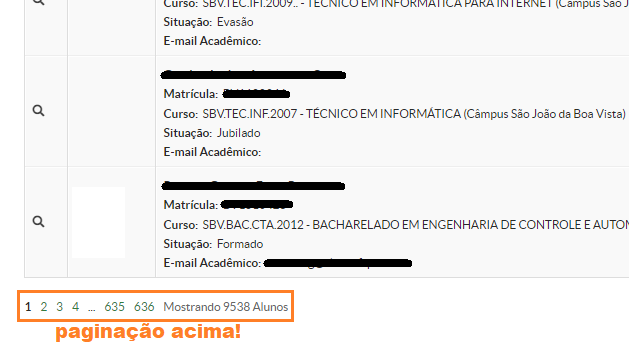
\includegraphics[scale=0.8]{imagens/cap08DesafioPaginacao}
        \\\textbf{Fonte:} Elaborada pelo autor
        \label{fig:cap08DesafioPaginacao}
    \end{figure}
    \FloatBarrier
\end{desafioSemArquivo}

\begin{desafioSemArquivo}{}{}{}
    Outra funcionalidade importante em sistemas reais é a emissão de relatórios ou de consultas personalizadas para a exibição de dados. Por exemplo, quero ter uma consulta de produtos em que eu insira parte da descrição de um produto em uma caixa de texto e, ao clicar no botão ``Consultar'', é mostrado na GUI do sistema todos os produtos que contenham na sua descrição o valor fornecido como uma substring. Pense só se o sistema tem centenas de produtos cadastrados e você precisa fazer uma venda! Imagine ficar rolando uma caixa de seleção por milhares de registro... Pois é, seu chefe gostou do seu trabalho na tarefa anterior e teu a missão de implementar essa funcionalidade no sistema. Ele quer que ao invés de ser exibida uma caixa de seleção com todos os produtos no formulário da venda, que haja um campo de texto onde o usuário fornecerá um valor que pode tanto ser o identificador do produto quanto seu código de barras e, ao teclar \destaque{\texttt{<ENTER>}} naquele campo, seja montada uma lista com os produtos obtidos, algo como mostrado na Figura~\ref{fig:cap08DesafioConsultaProduto}. Use sua imaginação e criatividade para implementar tal funcionalidade!
    
    \FloatBarrier
    \begin{figure}[!htbp]
        \centering
        \caption{Consulta de produtos no formulário de vendas}
        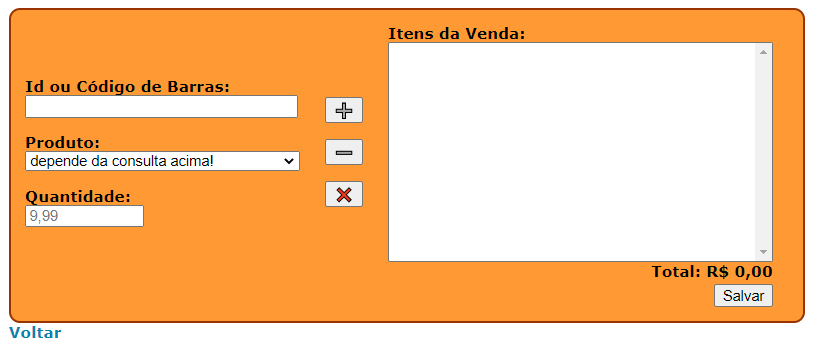
\includegraphics[scale=0.7]{imagens/cap08DesafioConsultaProduto}
        \\\textbf{Fonte:} Elaborada pelo autor
        \label{fig:cap08DesafioConsultaProduto}
    \end{figure}
    \FloatBarrier
\end{desafioSemArquivo}

\begin{desafioSemArquivo}{}{}{}
    Seu chefe adorou sua solução para o desafio anterior e agora quer mais um ``botãozinho'' no sistema. Entendedores entenderão hahaha! Ele quer que você implemente a emissão de relatórios para o sistema. Neste primeiro momento ele quer dois relatórios, um que mostre a quantidade vendida de todos os produtos em um período de tempo, ou seja, para cada produto, definindo-se uma data inicial e uma data final em um formulário, realizar a consulta no banco de dados e mostrar a quantidade que foi vendida de cada um desses produtos. O outro relatório é um relatório que mostre o montante total das vendas em um período, ou seja, ele quer saber quanto de dinheiro que entrou em um período de tempo. Você não precisa usar nada além do que já sabe, mas se quiser empregar o uso de alguma \textit{engine} de relatórios como o iReport\footnote{\url{https://community.jaspersoft.com/project/ireport-designer}}, fique à vontade. Fácil? Difícil? Seu emprego está em jogo! Mãos à obra!
\end{desafioSemArquivo}